\chapter{Infoturve}

\section{Korea isikukoodi näide}
2014. aastal tehti Lõuna-Koreas otsus vahetada välja isikukoodid\footnote{Lühike kokkuvõte ja edasisi viiteid saadaval siin \url{https://www.ria.ee/riigiarhitektuur/blog/2014/10/18/south-korea-about-to-overhaul-their-id-card/}}. Põhjuseks asjaolu, et sealne süstem oli üles ehitatud isikukoodi salajasusele. See viimane oli aga disainitud toetuma suhteliselt triviaalsetele turvameetmetele. Tulemuseks oli, et ühest küljest muutus isikukood ahvatlevaks ründeobjektiks ja teisalt olid rea intsidentide tulemusena kümne aasta jooksul sisuliselt kõigi kodanike isikukoodid lekkinud. Ja kuna identiteedivargus on üleüldine, tuleb isikukoodid välja vahetada.

\section{Infoturbe strateegiast}
Meid ümbritsevad infosüsteemid on muutunud ülimalt keeruliseks, organisatsioonid on erisugusest riist- ja tarkvarast põhjalikult läbi imbunud. Seetõttu on sisuliselt võimatuks muutunud täielik kontroll süsteemi üle. Heaks näiteks on väljakutsed BYOD\sidenote{\emph{Bring Your Own Device}, Too Oma Seade. Praktika, kus töötajad kasutavad töökeskkonnas isiklikke seadmeid. Tuntud ka kui \emph{Bring Your Own Disaster}, Too Oma Õnnetus} ümber ning sisuline võimekus tagada kogu organisatsioonis liikuva info varundamine. 

Samuti on tõsiasi, et kõigist paljudest komponentidest on mõni kogu aeg kas katki või siis ründele haavatav. Lahenduseks tundub olevat terviklik riskikäsitlus, sealhulgas süsteemi turvaliseks disainimine. Kuidas seda aga päriselt ilma kontolli omamata teostada? Head vastust anda ei ole, kui ehk võib abiks olla \citeauthor{leveson2011engineering}\cite{leveson2011engineering} ja tema mõtteviis ning arusaam, et keeruliste süsteemide puhul ei saa strateegiliselt eesmärgiks võtta totaalkaitset. Ehk, me ei ürita mitte kõiki süsteemi osa täielikult kontrollida ja kaitsta vaid maandame riskid \emph{piisavale} tasemele jättes teatud riskid teadlikult üles\sidenote{Avalikus sektoris on olukord teine. Seal ei saa asutus teadlikult aktsepteerida riski seadust rikkuda. Loomulikult jääb alati jääkrisk, millest me midagi ei tea, aga teadaolevat riski aktpseteerida ei saa. Kui me näiteks teame, et teatud krüptoalgoritm võib tulevikus murutud saada ja teame, et internetiliiklust salvestatakse, ei saa me näiteks rahvastikuregistrit selle algoritmi abil krüpteerituna internetti pidi edastada. Sest nii tehes võtame me riski avaldada isikuandmeid kolmandatele isikutele.}. 

Sedalaadi lähenemine eeldab aga ülevaadet süsteemi osadest, nende olulisusest süsteemi jaoks ning suhtelisest nõrkustest. Siit tuleneb aga jällegi küsimus süsteemi piiridest\index{Süsteem!Piirid}. Infoturbes lahendatakse probleem tüüpiliselt pragmaatiliselt: kui miski on oluliseks riski allikaks sellega ka tegeletakse.

Väga suurel määral sõltub infoturbega tegelemine infost (vt. ka \nameref{sec:valemid}). Järelikult on strateegiliselt oluline tegeleda riskide seirega. Ühest küljest tuleb jälgida oma süsteeme kuid vähemalt sama oluline on pidada silmas lähiümbruses (mis interneti mõistes ei tähenda loomulikult geograafilist lähedust) toimuvat. Siin on olulisel kohal mittetehniline seire: valdkonna kas avalikult või muul moel saada olev info tuleb pidevalt ohuhinnangute uuendamiseks ja prognooside tegemiseks läbi töötada. 

Eelnevat arvestades on selge, et infoturbe strateegia on tihedalt seotud paljude erinevate organisatsiooni toimimise aspektidega. OSA\sidenote{\emph{Open Security Architecture} on initsitatiiv, mis on eesmärgiks seadnud infoturbealase teadmuse avatud ja lihtsasti kasutatavateks mustriteks destilleerimise. Vt. \url{http://www.opensecurityarchitecture.org/cms/foundations/osa-taxonomy}} taksonoomia, kujutatud joonisel \ref{fig:osa} illustreerib seoseid ettevõtte strateegia, IT strateegia ja erinevate infoturbealaste tegevuste vahel. Tulemuseks on mõistete taksonoomia, mis võimaldab mõttestada infoturbe kohta organisatsioonilises kontekstis. Vaade on antud infosüsteemi vaatest, seega on näiteks kommunikatsioon pildilt puudu. 

\begin{figure}[h]
	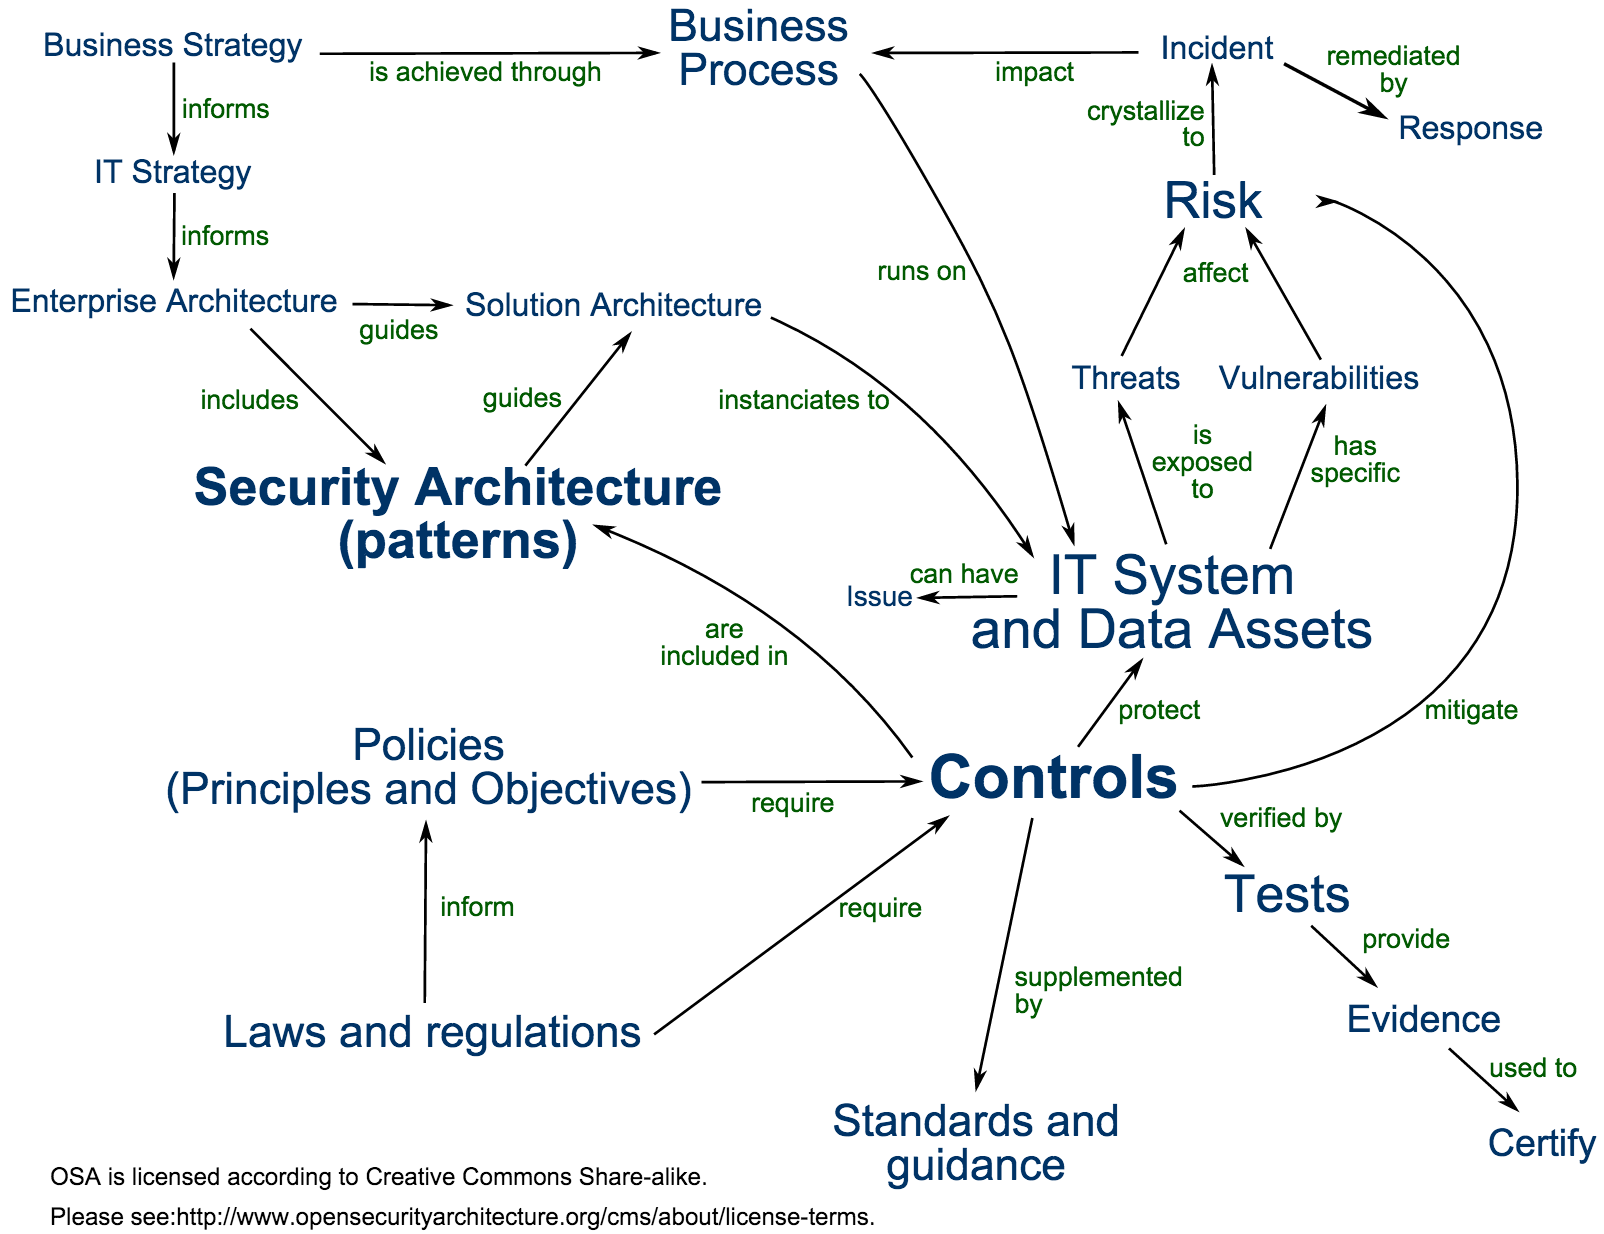
\includegraphics[width=\linewidth]{osa.png}%
	\caption{Seos äristrateegia ja infoturbe vahel OSA taksonoomia järgi} 
	\label{fig:osa}
\end{figure}

Sellel pildil on küll kesksel kohal infoturbe meetmed (\emph{Controls}), kuid sama olulised on erinevad infoturbe mustrid. Muster siinkohal on tavalisest üldisem mõiste tähendades suhteliselt üldist korratavat lahendust. Idee disainimustritest toodi esmakordselt välja füüsilise arhitektuuri valdkonnas\sidenote{\cite{alexander1977pattern} Paralleele infosüsteemide ja füüsilise ruumi planeerimise vahel on leitud ikka ja jälle. Mõnel juhul on nii üles ehitatud terveid metoodikaid:\cite{longepe2003enterprise}} ning OSA lähenemises on kesksel kohal infoturbe mustrite kataloog. Teine oluline tähelepanek on, et äristrateegiast tuleneb kaks olulist taksonoomia elementi: äriprotsessid, mida realiseerivad infosüsteemid ning EA\index{EA}, mis sisaldab infoturbe mustreid. Järelikult eeldab võimekus kaitsta infosüsteeme kooskõla äriprotsesside ja süsteemi arhitektuuri vahel. Mõistliku koostöö puudumine viib tõenäoliselt vastuolulini kus äriprotsess ei ole infoturbe mõistes kaitstav ärilises mõttes mõistliku määrani.

\section{Kuvandi olulisus infoturbes}
Nii valemi \ref{eq:tasuvus} (vt. lk \pageref{eq:tasuvus}) kui teiste riskimudelite puhul on olulisel kohal hinnangulisus. Ründajal on võimalik hinnata kohtuniku käitumist, õiguskaitse tõhusust ning kaitse taga asuva väärtust. Kuid tal ei ole võimalik neid teada. Järelikult on olulisel kohal infoturbes valemi parameetritest ebasoodsa mulje jätmine. Bütsantsi riik kasutas sama taktikat juba aastatuhandete eest, see toimib ka täna. Piltlikult öeldes võib seif olla valmistatud papist, kuid kuni kui kõik usuvad ta olevat läbimatust terasest, keegi talle kääridega ei lähene. Loomulikult on mulje ajutine ning raskesti juhitav ning seetõttu tuleb valmis olla selle purunemiseks. Kui levib info papist seifist, on maailmas kääre küllaga. Samuti ei ole ilmselt mõistlik tekitada kõrge väärtusega sihtmärgi kuvandit lisades ründest oodatavale kasule \enquote{feimi} komponendi.\sidenote{2013. aastal sundis Prantsuse DCRI, sealne spiooniorganisatsioon, prantsuskeelse Wikipedia toimetajat vahistamise ähvardusel muutma kogukonnateatmiku artiklit ühe Prantsuse õhujõudude raadiojaama kohta. Mispeale loomulikult too artikkel senisest võrratult rohkem tähelepanu sai. Tegu on niinimetatud Streisandi efektiga. 2003. aastal kabas Barbara Streisand kohtusse ühe fotograafi, kelle tehtud piltidelt (vt. joonis \ref{fig:barbara}) lauljatari häärber liiast kenasti kätte paistis. Enne kohtuasja oli pilte vaadatud mõned korrad, pärast kohtusse pöördumist on pilte ilmselt nähtud ilmselt sajad tuhanded huvilised.}

\begin{marginfigure}
	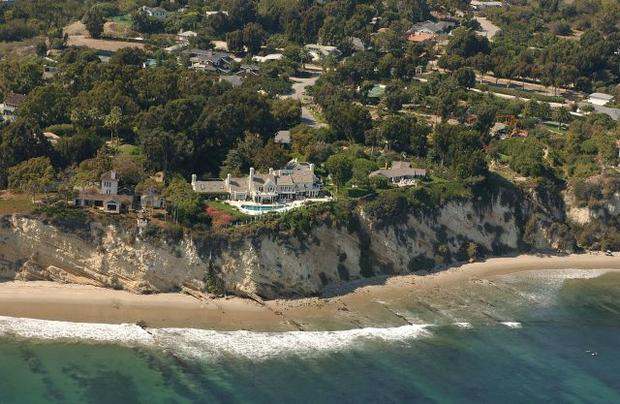
\includegraphics[width=\linewidth]{barbrara.jpg}%
	\caption{Barbara Streisandi villa Malibus. Kenneth and Gabrielle Adelman via Wikimedia Commons. CC BY-SA 3.0} 
	\label{fig:barbara}
\end{marginfigure}

Jättes kõrvale pideva automatiseeritud ründevoo, võetakse järgmised sihtmärgid kõige tõenäolisemalt ette:
\begin{itemize}
	\item Ettevõtted, millede ründamine on moraalselt õigustatav, mis kuuluvad \emph{fair game} kategooriasse
	\item Ettevõtted, millede kohta on alust arvata, et küberrünne võib teha märkimisväärset kahju
	\item Ettevõtted, millede ründamisel võib olla laiemaid tagajärgi väljaspool sihtmärki
\end{itemize}

\section{Rünnete tõsidus}
Eri liiki ründed võib tõsiduse järgi jagada neljaks tasemeks, iga järgnev on eelmisest tõsisem

\begin{enumerate}
	\item Käitlustõrge (näiteks (D)DoS\footnote{\emph{(Distributed) Denial of Service} on rünne, mille käigus ülekoormatakse tahtlikult teenust pakkuv taristu kas ühesest või hajutatud allikast}. Samas on tegemist kõige kõrgema profiiliga ründega, sest paistab lihtsasti välja. Kui teenus puudub, on see kohe kõigile näha
	\item Teenuste ja äritegevuse toimimine mittesoovitud moel. Näiteks Stuxnet, mis ei seisanud rünnatavaid seadmeid, vaid muutis nende tööre\v{z}iimi ning kuvas juhtimismoodulile ebakorrektset infot. Samasse kategooriasse kuulub rünne haigla infosüsteemi vastu millega muudetakse haigete diagnoose, veregruppe jne. 
	\item Teenuse ja äritegevuse usaldusväärsuse langetamine. Kui teenuse usaldusväärsus langeb alla kriitilise piiri, teenust ei kasutata. Seejuures ei ole oluline, kas ja mil määral andmete terviklus või konfidentsiaalsus tegelikult ohus on. Eesti e-riik on selles osas suurepäraseks näiteks: meie riigi toimimine sõltub suurel määral usaldusest terve e-ökosüsteemi (riiklikud institutsioonid, pangad, id-kaart, tehnilised lahendused jne) vastu 
	\item Kontrolli kaotamine teenuse või äritegevuse üle. Sel puhul võetakse üle andmed, kaob kontroll äriprotsesside toimimise üle, teenuste käideldavus kõigub jne.
\end{enumerate}

Arusaam rünnete tõsidusastmest on oluline eriti tänases pidevate rünnete kontekstis. Kuna keegi kogu aeg ründab on oluline keskendada ressursid tegelemaks kõrgema taseme rünnetega. Madalama taseme ründeid võib kas lihtsalt ignoreerida (kui oluline ikkagi on asutuse veebilehe kadumine internetist?) või rahuldaval määral automatiseerimise abil kontrolli alla võttes näiteks paigutades niigi avaliku veebilehe mõne teenusepakkuja elastsesse pilve.

\section{Infoturbe valemid} 
\label{sec:valemid}
\subsection{Ründe tasuvus}
\begin{equation}
		S_p>P_f(S_a + P_c S_c)
		\label{eq:tasuvus}
\end{equation}

	\begin{description}
		\item[$S_p$] Ründest oodatav kasu
		\item[$P_f$] Ründe ebaõnnestumise tõenäosus
		\item[$S_a$] Ründe läbi viimise kulu
		\item[$P_c$] Vahele jäämise tõenäosus
		\item[$S_c$] Vahele jäämise kulu
	\end{description}

Toodud valemi puhul on oluline silmas pidada kahte asjaolu. 

Esiteks, et ründe ebaõnnestumise tõenäosus on reaalselt alati väiksem kui üks. Põhjuseks lihtsalt sotsiotehniliste süsteemide ülikeerukas olemus. Sihitud ja hoolikalt kavandatud ründe puhul ei ole küsimus selles, kas kaitsest suudetakse läbi murda. Küsimus on selleks kuluvas ajas ja ressursis ning läbimurde sügavuses. Silmas tuleb pidada ka ründevektori "ülevoolavust": alati valitakse ründeks kõige madalama kulu/tulu suhtega vektor. Süsteemide turvalisuse tõstmisega teatud piirist edasi suureneb lihtsalt sotsiaalrünnete surve ning süsteemi kui terviku turvalisus ei tõuse. 

Teiseks, muutujad on alati hinnangulised, neid ei ole ründajal võimalik otseselt mõõta. Siit tuleneb vajadus mõista ründajaid. Tegu on ju lõpuks nende poolt antud hinnangutega. Et eri osapoolte suhtelised võimekused ja huvid on erinevad, on erinevad ka nende hinnangud kulule ning ründest oodatavale kasule. On ju vahe, kas ründajaks on grupp internetiotsingut valdavaid teismelisi või mõne riigi APT\footnote{\emph{Advanced Persistent Threat} on varjatud ja pideva kübersurve oht, mis on suunatud konkreetse ospoole vastu} spetsialistid. 

Kuna evolutsioon dikteerib kõigi osapoolte huvi maksimeerida kasu minimeerides kahju võimaldab ründe tasuvuse analüüs hinnata kõige tõenäolisemaid sihtmärke ning seega planeerida kaitset: kuhu ja kui kõrged müürid ehitada. 

\subsection{Riski hinnang}

\begin{equation}
	RISK(Threat) = Threat \times Consequence \times Vulnerabilities
	\label{eq:risk}
\end{equation}

\begin{description}
	\item[RISK] hinnang riskile
	\item[Threat] hinnang ohule
	\item[Consequence] hinnang riski ohu realiseerumise tagajärgedele
	\item[Vulnerabilities] hinnang süsteemi haavatavusele
\end{description}

Valem \ref{eq:risk} ütleb, et risk on mittelineaarses sõltuvuses ohust, selle realiseerumise tõenäosusest ning süsteemi haavatavusest. Ehk, madala tõenäosuse kuid suure mõjuga oht, millele ollakse haavatavad on sama oluline kui kõrge tõenäosuse ja suure mõjuga oht, mille vastu ollakse hästi kaitstud. Samuti nähtub siit, et iga elemendi nulli viimine viib nulli ka riski. 

Nagu ka valemi \ref{eq:tasuvus} puhul, on siin tegu hinnangutega. Kuid erinevalt ründe tasuvusest on siin ebatäpne mulje pigem probleem, kui lahendus. Kui, eelnevalt kasutatud analoogiat jätkates, seif on papist, on seda kasulik teada ning mitte uskuda teda terasest olevat. Vastasel juhul on oht haavatavust alahinnata. Sama kehtib ka tagajärgede ja ohu kohta. Järelikult on täpne ning teadmistepõhine teadmine olukorrast adekvaatse riskijuhtimise puhul ülioluline.

Absoluutskaalade asemel võib valemi muutujate hindamisel kasutada suhtelisi. Näiteks võib toimida nii:

\begin{enumerate}
	\item Loetle ohud
	\item Anna igale ohule ohuhinnang skaalal 1-10
	\item Anna igale ohule sama skaalat kasutades tagajärje hinnang. Seejuures kata kinni ohuhinnang tagamaks muutujate sõltumatus
	\item Anna igale ohule haavatavushinnang kasutades jällegi sama skaalat ja kattes teised hinnangud kinni
\end{enumerate}

Nüüd oled igale ohule saanud suhtelise riskihinnangu, mis võimaldab neid sorteerida, valida maandamiseks jne.  

\subsection{Alternatiivide kaalumine}
\begin{equation}
	(B_1 - E_1) - (B_2 - E_2) > RISK(\varepsilon_1)-RISK(\varepsilon_2)
	\label{eq:alternative}
\end{equation}

\begin{description}
	\item[B] Kasu alternatiivi rakendamisest
	\item[E] Alternatiivi rakendamisega seotud kulud, sealhulgas riskide maandamiseks tehtavad kulud 
	\item[$\varepsilon$] Jääkoht, ehk ohud mis säilivad pärast kõigi meetmete rakendamist
\end{description}

Kuigi tavaliselt kasutatakse samalaadset valemit äriprojektide hindamisel (kasu peab üles kaaluma riskid) siis valemit \ref{eq:alternative} saab kasutada alternavtiivide hindamiseks. Siinjuures on oluline aru saada, et riski saab liigutada võrratuse paremalt poolelt vasakule ja vastupidi tehes või vähendades kulutusi jääkriski vähendamiseks või suurendamiseks. Teine kriitiline punkt siinkohal on ajaline mõõde: nii $B$, $E$ kui $RISK(\varepsilon)$ tuleb arvutada nüüdisväärtusena.

Olgu meil näiteks küsimus, kas võime oma andmeid hoida avaliku pilveteenuse pakkuja juures. Sel juhul 
\begin{itemize}
	\item $B_1-E_1$ on hinnang oma serverite pidamisest saadud kasule, millest on lahutatud serverite majutamise kulud (sealhulgas riskide maandamisele tehtavad kulutused). Kui oma serverite hoidmine iseensest tulu ei teeni, siis võib arvestada, et $B_1=0$. 
	\item $B_2-E_2$ on hinnang pilveteenusest saadavale kasule, millest on lahutatud tehtavad kulutused mis jällegi koosnevad nii riskide maandamiseks tehtavatest kuludest kui ka perioodilisest arvest. Jällegi, kui pilveteenus iseensest näiteks läbi parema käideldavuse kasu ei too, siis $B_2=0$
	\item $\varepsilon_1$ on jääkoht juhul, kui servereid majutatakse ise
	\item $\varepsilon_2$ on jääkoht pilveteenuse majutamise puhul
\end{itemize}

Pilve puhul me tõenäoliselt leiame, et riskid suurenevad, tekib teatav lisandväärtus ja kulud vähenevad. Küsimust pilve kasutamisest saab aga positiivselt otsustada vaid juhul, kui võrratus kehtib ning meie tegevuse tulud ületavad jätkuvalt riske.


\subsection{Oodatav kahju} 

	\begin{align}
		Annualised\ Expected\ Loss &= Frequency\ of\ a\ given\ attack\ type \label{eq:loss}\\
		&\times Potential\ Loss \nonumber \\
		&\times Extent\ to\ which\ the\ loss\ occurs \nonumber
	\end{align}


\begin{description}
	\item[Annualised Expected Loss] Oodatav aastane kahju
	\item[Frequency of a given attack type] Konkreetset liiki ründe esinemissagedus
	\item[Potential loss] Potentsiaalne kahju ründest
	\item[Extent to which the loss occurs] Potentsiaalne kahju keskmine realiseerumise määr
\end{description}

Valem \ref{eq:loss} võimaldab hinnata oodatavat kahju ründest. Teades, kui tihti ründed esinevad\footnote{Rünnete esinemise jaotus ning selle hindamine sisuliselt pidevate rünnete tingimustes on keeruline valdkond, millesse siinkohal liigne süveneda}, mis on neist tekkida võiv kahju ning mil määral kahju tavaliselt realiseerub, võib hinnata tekkivat kogukahju. Näiteks, kui meil on keskmiselt kaks tõsisemat teenustõrkerünnet aastas, mis kumbki võivad tekitada 10 000.- \euro kahju ning eelnev kogemus võimaldab hinnata, et kümmekond protsenti kahju õnnestub ära hoida on oodatav kahju $E(L)=2 \times 10000 \times .9 = 18 000$. 

Tegu ei ole infoturbespetsiifilise valemiga, täpselt samuti hinnatakse näiteks krediidiriske.

\section{Pilveriskidest}
Pilv kui kellegi teise arvuti ja mitte arvuti puudumine
\TODO täida sisuga. 

\section{Küsimusi aruteluks}
\subsection{Kuidas tellida turvalist tarkvara?}
\TODO: täida sisuga
Kui turvalisus ei ole süsteemi funktsioon vaid emergentne omadus, siis mida see tähendab tellimise jaoks? Emergents ei ole ju lõpuni ennustatav.

Saalist
\begin{itemize}
	\item Tee endale selgeks, mida kaitsta. Ja miks. Määra turvatase
	\item Rakenda elementaarsed hügieeninõuded toetudes standardile (OWASP näiteks)
\end{itemize}


\section{Lahti kirjutada}
Cakery Levier IT case. Retseptid füüsiliselt näha. Kultuuri kaotamise risk läbi IT rakendamise (laoarvestus vs. lastele küpsiste pakkumine)

